\documentclass{article}
\usepackage[utf8]{inputenc}
\usepackage[russian]{babel}
%\usepackage{systeme}
\usepackage{amsmath}
\usepackage{amssymb}
\usepackage{amsfonts}
\usepackage{mathtext}


%\usepackage[dvips]{graphicx}
\usepackage[final]{graphicx}
\graphicspath{{noiseimages/}}

\renewcommand{\baselinestretch}{1.5}

\title{Четвертое задание по БМСО}
\author{Ярослав Аверьянов}
\date{Ноябрь 2015}

\begin{document}

\maketitle

\section{Первая задача}
Плотность случайной величины с центрированным распределением Коши при $y \in \mathbf{R}$:
\begin{center}
$p(y) = \frac{1}{\pi}\frac{1}{c(1 + \frac{y^2}{c^2})}, c > 0$
\end{center}
Приведем пример преобразования $\phi(x), x \in [0,1] : \phi(X)$ - СВ с распределением Коши при $X \sim \mathbf{U}[0,1]$.\\
Возьмем
\begin{center}
$\phi(X) = C \cdot tg(\pi(X - \frac{1}{2}))$
\end{center}
$p_{\phi}(z) = \frac{d}{dz}F_{\phi}(z) = \frac{d}{dz}\mathbf{P}[C\cdot tg(\pi(X - \frac{1}{2})) \leq z] = \frac{d}{dz} \mathbf{P}[X \leq \frac{1}{\pi}arctg(\frac{z}{c}) + \frac{1}{2}] = \frac{d}{dz} \int_{0}^{\frac{1}{\pi}arctg\frac{z}{c} + \frac{1}{2}} dx = \frac{1}{\pi} \cdot \frac{d}{dz}(arctg(\frac{z}{c}) + \frac{\pi}{2}) = \frac{1}{\pi c(1 + (\frac{z}{c})^2)}$.\\
Преобразование $\phi(X)$ - не единственное, т.к. $1 - X \sim U[0,1] \to \phi(X) = \phi(1 - X)$.

\section{Вторая задача}
Рассматривается полуэллипсоид в $3D$, заданный параметрически:\\
$
\begin{cases}
x = \sqrt{3}sin(\theta)cos(\phi), \\
y = \sqrt{2}sin(\theta)sin(\phi), \\
z = cos(\theta)
\end{cases}
$\\
$\theta \in [0,\pi/2], \phi \in [0,2\pi].$\\
Используем метод rejection sampling и равномерное на $[0, \pi/2]\times[0,2\pi]$
Площадь заданного полуэллипсоида $\Omega$ задается как:
\begin{center}
$S = \iint_{\Omega} \sqrt{EG - F^2}d\theta d\phi,$
\end{center}
Коэффиценты:\\
$E = (x_{\theta}^{'})^2 + (y_{\theta}^{'})^2 + (z_{\theta}^{'})^2$\\
$F = x_{\theta}^{'}x_{\phi}^{'} + y_{\theta}^{'}y_{\phi}^{'} + z_{\theta}^{'}z_{\phi}^{'}$\\
$G = (x_{\phi}^{'})^2 + (y_{\phi}^{'})^2 + (z_{\phi}^{'})^2$\\
Плотность равномерного распределения на поверхности полуэллипсоида:
\begin{center}
$p(\theta, \phi) = \frac{1}{S} \sqrt{EG - F^2},$
\end{center}
Здесь $EG - F^2 = (2sin^2(\theta)cos^2(\phi) + 3sin^2(\theta)sin^2(\phi))(2cos^2(\theta)sin^2(\phi) + 3cos^2(\theta)cos^2(\phi) + sin^2(\theta)) - sin^2(\theta)sin^2(\phi)cos^2(\theta)cos^2(\phi)$
\begin{center}
$\sqrt{EG - F^2} = Sp(\theta,\phi) \leq \sqrt{3}$ на $[0,\pi/2]\times [0,2\pi]$
\end{center}

\begin{figure}[h]
\center{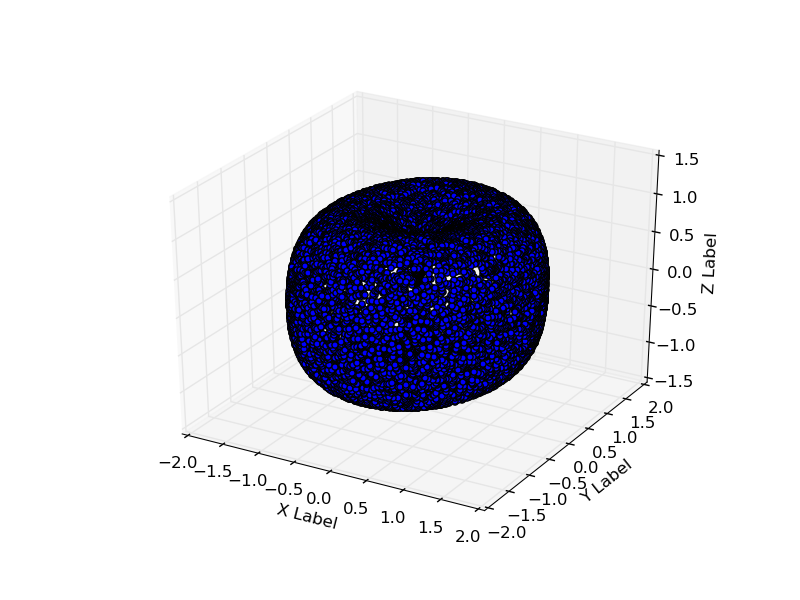
\includegraphics[width=1\linewidth]{surf}}
\caption{Our surface}
\label{ris:image}
\end{figure}

Применим алгоритм rejection sampling:\\
1.Сэмплируем $\theta \sim \mathbf{U}[0,\pi/2], \phi \sim \mathbf{U}[0,2\pi]$.\\
2.Сэмлируем $\gamma \sim \mathbf{U}[0, \sqrt{3}]$.\\
3.Вычисляем $Sp(\theta,\phi)$:\\
a)Если $\gamma \leq Sp(\theta,\phi), \to $ принимаем $(\theta, \phi)$.\\
б)Если $\gamma > Sp(\theta, \phi), \to $ отклоняем $(\theta, \phi)$.\\

Получились следующие графики:
\begin{figure}[h]
\center{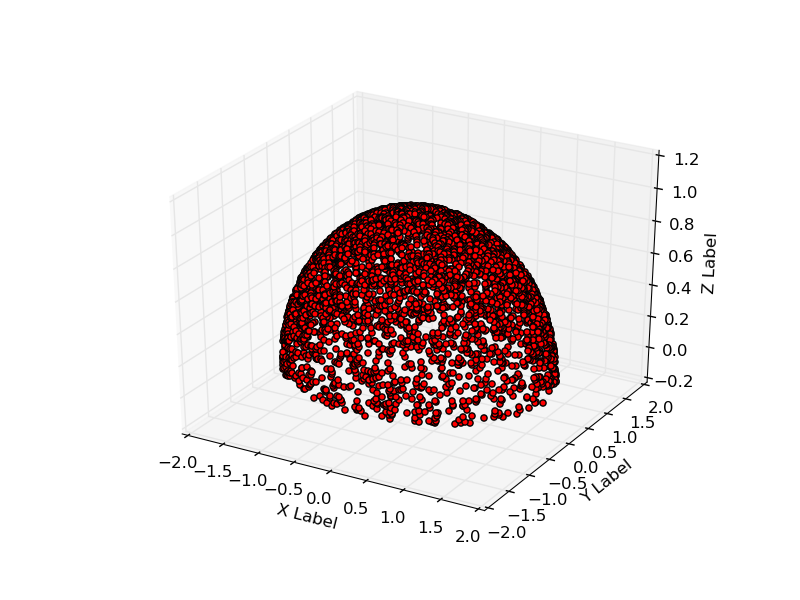
\includegraphics[width=0.7\linewidth]{figure_1}}
\caption{5000 точек}
\label{ris:image}
\end{figure}

\begin{figure}[h]
\center{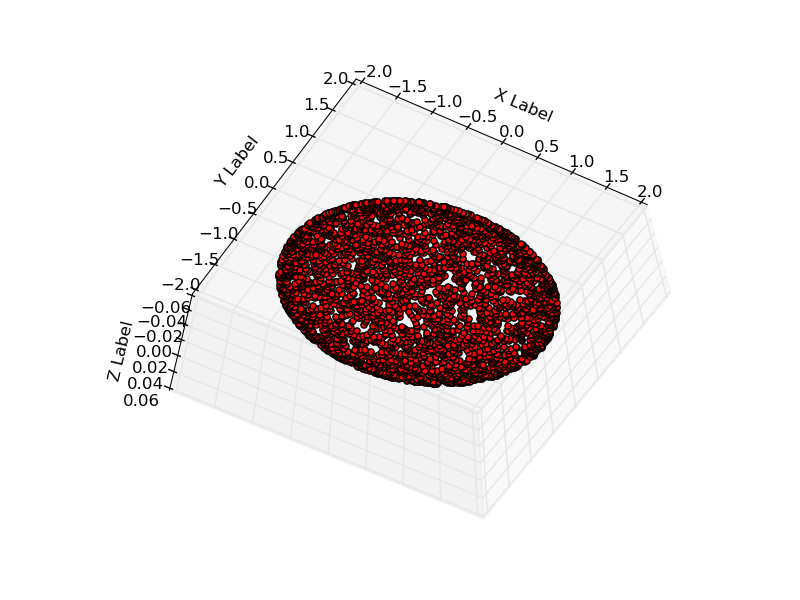
\includegraphics[width=0.7\linewidth]{figure_2}}
\caption{5000 точек, вид сверху}
\label{ris:image}
\end{figure}

\begin{figure}[h]
\center{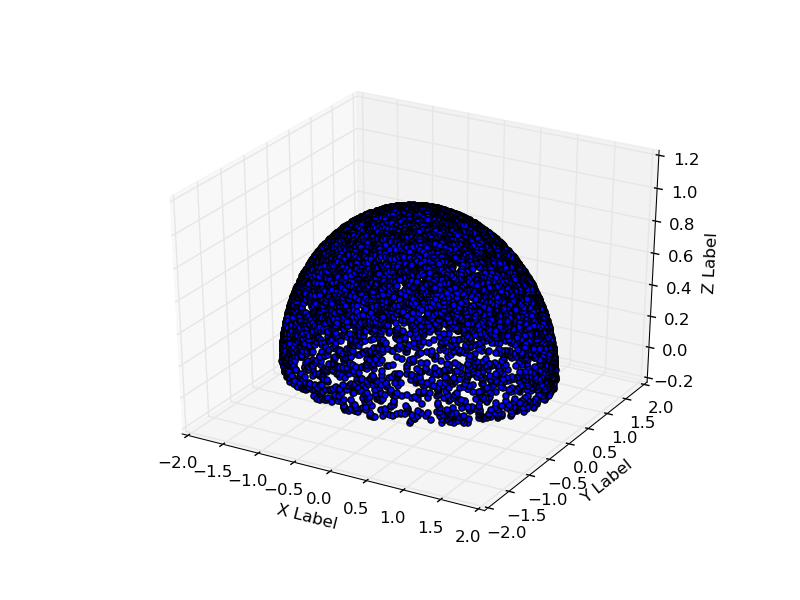
\includegraphics[width=0.7\linewidth]{figure_1-1}}
\caption{10000 точек}
\label{ris:image}
\end{figure}

\begin{figure}[h]
\center{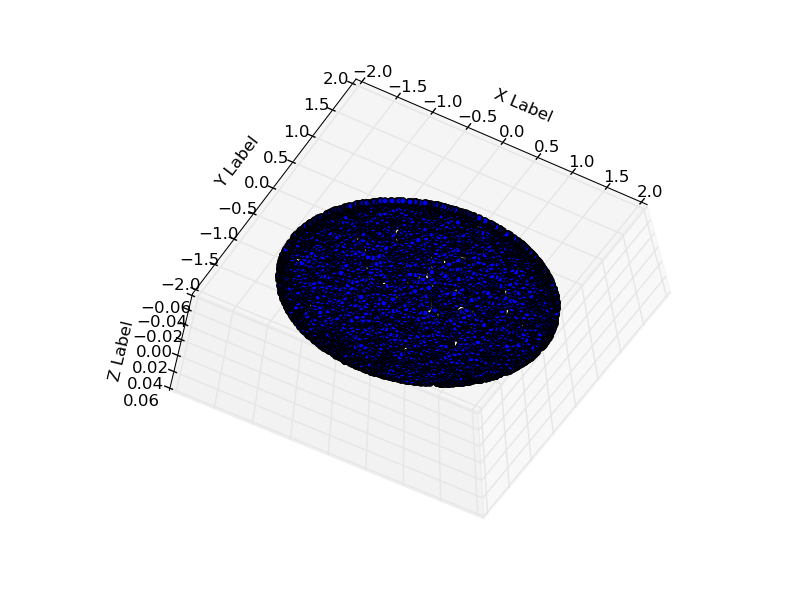
\includegraphics[width=0.7\linewidth]{figure_2-1}}
\caption{10000 точек, вид сверху}
\label{ris:image}
\end{figure}



\end{document}